\documentclass{article}
\usepackage{fullpage}
\usepackage{amsmath}
\usepackage{amsfonts}
\usepackage{tipa}
\usepackage{tikz}
\newcommand\myeq{\mathrel{\stackrel{\makebox[0pt]{\mbox{\normalfont\tiny def}}}{=}}}
\begin{document}
\begin{center}
\Large{A Kikuyu Christmas}
\end{center} 
\vspace{.5cm} 
\par \indent
This short writeup will offer a logical transduction on autosegmental representations of tone shift in Kikuyu, which has been proven to be MSO-undefinable under certain assumptions (Jardine 2017). The key with characterizing these alternations is assuming underlying associations between tones and TBUs for individual monosyllabic morphemes.\\
\indent
Consider an idealized form such as [on+ni+i+ni] 'smallness' (see Clements and Ford 1979: 197), with an output form like below:\\
\begin{center}
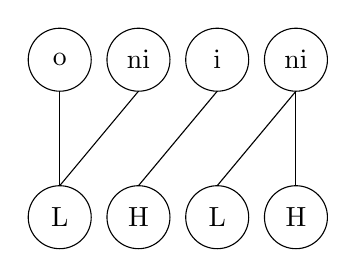
\begin{tikzpicture}
	\draw (-2,2) circle [radius = .4] node {o};
	\draw (-1,2) circle [radius = .4] node {ni};
	\draw (0,2) circle [radius = .4] node {i};
	\draw (1,2) circle [radius = .4] node {ni};
	\draw (-2,0) circle [radius = .4] node {L};
	\draw (-1,0) circle [radius = .4] node {H};
	\draw (0,0) circle [radius = .4] node {L};
	\draw (1,0) circle [radius = .4] node {H};
	\draw [-] (-2,1.6) -- (-2,.4);
	\draw [-] (-1,1.6) -- (-2,.4);
	\draw [-] (0,1.6) -- (-1,.4);
	\draw [-] (1,1.6) -- (0,.4);
	\draw [-] (1,1.6) -- (1,.4);
\end{tikzpicture}\\
\smallskip{}
Figure 1: [o+ni+i+ni] Output Form
\end{center}
The first and second [L] tones and the first [H] tone are said to \textit{shift} one syllable to the right, with well-formedness conditions determining the subsequent tone to TBU associations. Recent work by Jardine (2017) has proven that, under certain assumptions, tone shift in Kikuyu is MSO-undefinable. Positing underlying associations between tones and TBUs on individual morphemes (as below), however, characterizing Kikuyu tone shift is well within the MSO threshold.\\
\begin{center}
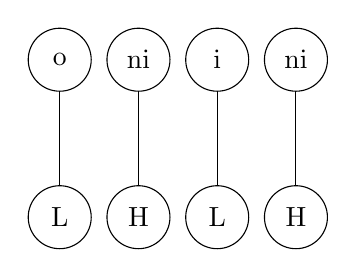
\begin{tikzpicture}
	\draw (-2,2) circle [radius = .4] node {o};
	\draw (-1,2) circle [radius = .4] node {ni};
	\draw (0,2) circle [radius = .4] node {i};
	\draw (1,2) circle [radius = .4] node {ni};
	\draw (-2,0) circle [radius = .4] node {L};
	\draw (-1,0) circle [radius = .4] node {H};
	\draw (0,0) circle [radius = .4] node {L};
	\draw (1,0) circle [radius = .4] node {H};
	\draw [-] (-2,1.6) -- (-2,.4);
	\draw [-] (-1,1.6) -- (-1,.4);
	\draw [-] (0,1.6) -- (-0,.4);
	\draw [-] (1,1.6) -- (1,.4);

\end{tikzpicture}\\
\smallskip{}
Figure 2: [o+ni+i+ni] Underlying Form
\end{center}
Since associations between tones and TBUs are specified underlyingly, this will require an input signature that specifies the binary association relation. There will also be an output association relation in the output signature, in addition to the unary tone and syllable relations as well as the successor relation, as shown below:
\begin{center}
\begin{tabular}{l}
$\langle D; \triangleleft, P_{\sigma}, P_{H}, P_{L}, \circ \rangle$\\
$\langle D'; \triangleleft_{o}, R_{\sigma}, R_{H}, R_{L}, \circ_{o} \rangle$\\
\end{tabular}
\end{center}
It will also be necessary to define predicates which identify the first and last elements on a tier:
\begin{center}
$\varphi_{\mathsf{initial}}(x) \myeq \forall y [ (x < y)]$\\
$\varphi_{\mathsf{final}}(x) \myeq \forall y [ (y < x)]$
\end{center}
The copy set is set to {1}; the output copy will contain two tiers.\\
The next step is to define the output unary relations. These are defined in terms of the input relations:
\begin{center}
\begin{tabular}{l}
$R^{1}_{\mu}(x) \myeq P_{\mu}(x)$\\
$R^{1}_{H}(x) \myeq P_{H}(x)$\\
$R^{1}_{L}(x) \myeq P_{L}(x)$\\
\end{tabular}
\end{center}
The association relation on the first copy set is defined as below; the variable $x$ refers to TBUs and $y$ to tonal segments.
\begin{center}
$x \circ^{1,1}_{o} y \myeq (\exists x'[ x \triangleleft x' \wedge x' \circ y]) \vee ( \mathsf{initial}(x) \wedge \mathsf{initial}(y)) \vee (\varphi_{H}(y) \wedge \mathsf{final}(y) \wedge \mathsf{final}(x))$
\end{center}
The output association relation comprises three disjuncts. The first disjunct is analogous to Clements and Ford's ITAR2 and WFC1, that is, a TBU associates to the tonal segment which associates to its immediate predecessor in the input (the rightward shift), and this process iterates throughout an entire surface form. The second disjunct corresponds to WFC3, which associates the unassociated initial tonal segment to the first TBU. Finally, the third disjunct represents the High Tone Association rule, driving association between word-final high tones to word-final TBUs.
The input and output forms for [o+ni+i+ni] are represented in Figure 3.\\
\begin{center}
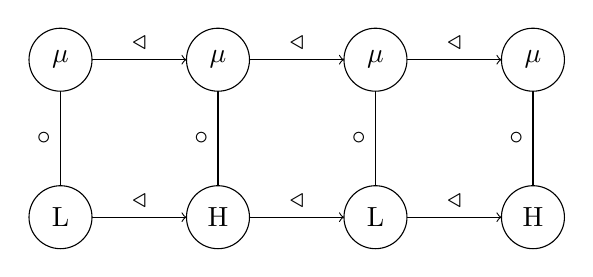
\begin{tikzpicture}
	\draw (-4,2) circle [radius = .4] node {$\mu$};
	\draw (-2,2) circle [radius = .4] node {$\mu$};
	\draw (0,2) circle [radius = .4] node {$\mu$};
	\draw (2,2) circle [radius = .4] node {$\mu$};
	\draw (-4,0) circle [radius = .4] node {L};
	\draw (-2,0) circle [radius = .4] node {H};
	\draw (0,0) circle [radius = .4] node {L};
	\draw (2,0) circle [radius = .4] node {H};
	\draw [->] (-3.6,2) -- (-2.4,2) node [above, pos = .5] {$\triangleleft$};
	\draw [->] (-3.6,0) -- (-2.4,0) node [above, pos = .5] {$\triangleleft$};
	\draw [->] (-1.6,2) -- (-0.4,2) node [above, pos = .5] {$\triangleleft$};
	\draw [->] (-1.6,0) -- (-0.4,0) node [above, pos = .5] {$\triangleleft$};
	\draw [->] (0.4,2) -- (1.6,2) node [above, pos = .5] {$\triangleleft$};
	\draw [->] (0.4,0) -- (1.6,0) node [above, pos = .5] {$\triangleleft$};
	\draw [-] (-2,1.6) -- (-2,.4) node [left, pos = .5] {$\circ$};
	\draw [-] (-4,1.6) -- (-4,.4) node [left, pos = .5] {$\circ$};
	\draw [-] (-0,1.6) -- (-0,.4) node [left, pos = .5] {$\circ$};
	\draw [-] (2,1.6) -- (2,.4) node [left, pos = .5] {$\circ$};
\end{tikzpicture}\\
\vspace{1.5cm}
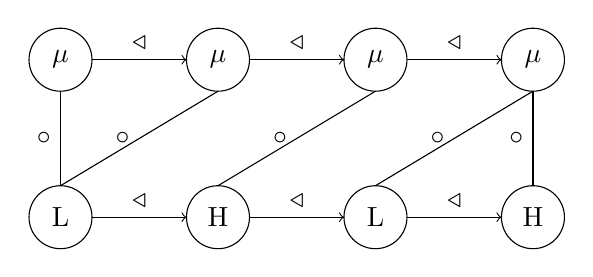
\begin{tikzpicture}
\draw (-4,2) circle [radius = .4] node {$\mu$};
	\draw (-2,2) circle [radius = .4] node {$\mu$};
	\draw (0,2) circle [radius = .4] node {$\mu$};
	\draw (2,2) circle [radius = .4] node {$\mu$};
	\draw (-4,0) circle [radius = .4] node {L};
	\draw (-2,0) circle [radius = .4] node {H};
	\draw (0,0) circle [radius = .4] node {L};
	\draw (2,0) circle [radius = .4] node {H};
	\draw [->] (-3.6,2) -- (-2.4,2) node [above, pos = .5] {$\triangleleft$};
	\draw [->] (-3.6,0) -- (-2.4,0) node [above, pos = .5] {$\triangleleft$};
	\draw [->] (-1.6,2) -- (-0.4,2) node [above, pos = .5] {$\triangleleft$};
	\draw [->] (-1.6,0) -- (-0.4,0) node [above, pos = .5] {$\triangleleft$};
	\draw [->] (0.4,2) -- (1.6,2) node [above, pos = .5] {$\triangleleft$};
	\draw [->] (0.4,0) -- (1.6,0) node [above, pos = .5] {$\triangleleft$};
	\draw [-] (-4,1.6) -- (-4,.4) node [left, pos = .5] {$\circ$};
	\draw [-] (2,1.6) -- (2,.4) node [left, pos = .5] {$\circ$};
	\draw [-] (-4,.4) -- (-2,1.6) node [left, pos = .5] {$\circ$};
	\draw [-] (-2,.4) -- (0,1.6) node [left, pos = .5] {$\circ$};
	\draw [-] (0,.4) -- (2,1.6) node [left, pos = .5] {$\circ$};
\end{tikzpicture}\\
\smallskip{}
Figure 3: [o+ni+i+ni] Input and Output Forms 
\end{center}
\pagebreak
\begin{center} References \end{center}
\smallskip{}
\hangindent=.5cm
Clements, George and Kevin Ford. 1979. Kikuyu tone shift and its synchronic consequences. \textit{Linguistic Inquiry} 10,2: 197-210.\\
\par \noindent
Jardine, Adam. 2016. Autosegmental representations in Zigula and Shambaa. Ms, Rutgers.\\
\par \noindent
\hangindent=.5cm
Jardine, Adam. 2017. On the logical complexity of autosegmental representations. \textit{Proceedings of the 15th Meeting on the Mathematics of Language}: 22-35.\\
\end{document}
